\chapter{Floating point arithmetic}
The next defintion take from \cite{lefevre2004arithmetique}, \cite{markstein2008new} and \cite{muller2010handbook}.
\section{Definitions}
\begin{defin}:
\textbf{Floating point} is a way of writing real numbers. This expression is mostly used for computers. It is different from the fixed point. It is represented with a precision,  base(radix),  sign,  mantissa and exponent.\\ 
Let $x$ be a real number, so in this way we have $x = s.M.\beta^{e-p+1}$ with $s$ the \textbf{sign}, $M$ the \textbf{mantissa}, $\beta$ a \textbf{base}(\textbf{radix}), $e$ the \textbf{exponent} and $p$ the \textbf{precision}.
 \end{defin}
 $p$ represents the number of bits of the \textbf{mantissa}.
 In our research, we prefer to use $E = e - bias$ to be possible to have a negative exponent and also to have $E_{min}= 1 - E_{max}$.\\ 


Floating points are composed of several precisions given by the \textbf{IEEE 754} standard.\\

The next defintion take from \cite{enwiki:1096894205}.
\begin{defin} :
\textbf{IEEE 754} is a floating point standard created by \textbf{the Institute of Electrical and Electronics Engineers}. It is the  most used standard for computer calculations .
This standard imposes formats for each floating number with its representations of sign, mantissa, exponent and also the five rounding modes used.
\end{defin}

\textbf{IEEE 754-2008} defines three possible formats for base of $2$ of \textbf{floating point}: \textbf{Binary32}, \textbf{Binary64} and \textbf{Binary128}.

\begin{itemize}
    \item \textbf{Binary32} (\textbf{single precision}) (Figure $\ref{fig:B32}$) :\\ 
    \textbf{Binary32} is stored on $32$ bits, with $1$ bit for the \textbf{sign}, $8$ bits for the \textbf{exponent} and $23$ bits for the \textbf{mantissa} without its strong bit ($24$ bits). 
    
    \item \textbf{Binary64} (\textbf{double precision}) (Figure $\ref{fig:B64}$) :\\
    \textbf{Binary64} is stored on $64$ bits, with $1$ bit for the \textbf{sign}, $11$ bits for the \textbf{exponent} and $52$ bits for the \textbf{mantissa} without its strong bit ($53$ bits). 
    
    
    \item \textbf{Binary128} (\textbf{Quadruple precision}) (Figure $\ref{fig:B128}$) :\\
    \textbf{Binary128} is stored on $128$ bits, with $1$ bit for the \textbf{sign}, $15$ bits for the \textbf{exponent} and $112$ bits for the \textbf{mantissa} without its strong bit ($113$ bits). 
\end{itemize}

In the $3$ Schematics below of the $3$ formats, we have the leftmost bit is the strong bit and the rightmost is the weakest bit:
\begin{figure}[H]
    \centering
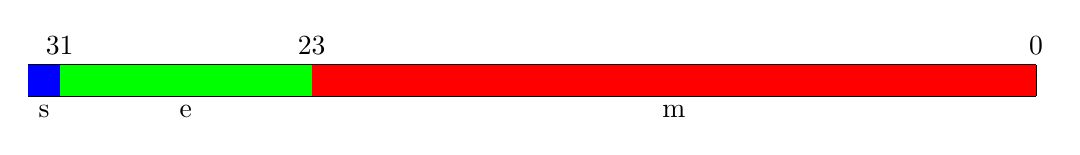
\begin{tikzpicture}
      \draw[step=0.4cm, black,  thin] (0, 0) grid (12.8, 0.4);   
     \fill [blue](0,0) rectangle(0.4,0.4);
     \fill [green](0.4,0) rectangle(3.6,0.4);
     \fill [red](3.6,0) rectangle(12.8,0.4);
     \draw (0.2,0) node[below] {s}  ;
     \draw (2,0) node[below] {e}  ;
     \draw (8.2,0) node[below] {m}  ;
     \draw (0.4,0.4) node[above]{31};
     \draw (3.6,0.4) node[above]{23};
     \draw (12.8,0.4) node[above]{0};
\end{tikzpicture}
\caption{Binary32}
\label{fig:B32}
\end{figure}
\begin{figure}[H]
    \centering
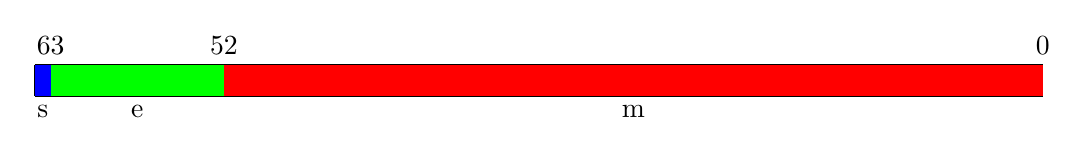
\begin{tikzpicture}
     \draw[step=0.4cm, black,  thin] (0, 0) grid (12.8, 0.4);   
     \fill [blue](0,0) rectangle(0.2,0.4);
     \fill [green](0.2,0) rectangle(2.4,0.4);
     \fill [red](2.4,0) rectangle(12.8,0.4);
     \draw (0.1,0) node[below] {s}  ;
     \draw (1.3,0) node[below] {e}  ;
     \draw (7.6,0) node[below] {m}  ;
     \draw (0.2,0.4) node[above]{63};
     \draw (2.4,0.4) node[above]{52};
     \draw (12.8,0.4) node[above]{0};
\end{tikzpicture}
\caption{Binary64}
\label{fig:B64}
\end{figure}
\begin{figure}[H]
    \centering
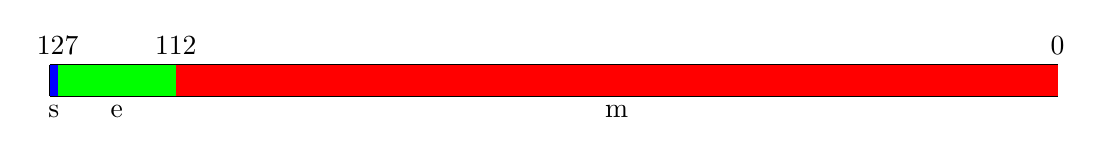
\begin{tikzpicture}
     \draw[step=0.4cm, black,  thin] (0, 0) grid (12.8, 0.4);   
     \fill [blue](0,0) rectangle(0.1,0.4);
     \fill [green](0.1,0) rectangle(1.6,0.4);
     \fill [red](1.6,0) rectangle(12.8,0.4);
     \draw (0.05,0) node[below] {s}  ;
     \draw (0.85,0) node[below] {e}  ;
     \draw (7.2,0) node[below] {m}  ;
     \draw (0.1,0.4) node[above]{127};
     \draw (1.6,0.4) node[above]{112};
     \draw (12.8,0.4) node[above]{0};
\end{tikzpicture}
\caption{Binary128}
\label{fig:B128}
\end{figure}     
We also have \textbf{Binary80} which is an \textbf{extended double precision} and two others possible formats for base of $10$:
 \begin{itemize}
     \item  \textbf{decimal64} is stored on $64$ bits.
     \item  \textbf{decimal128} is stored on $128$ bits.
 \end{itemize}
In \textbf{C} programming, \textbf{Binary32} represents \textbf{Float}, \textbf{Binary64} is \textbf{Double}, \textbf{Binary80} is \textbf{long-double} and \textbf{Binary128} is \textbf{float128}.\\
Throughout our research, we will only use \textbf{Binary64}.\\
The real numbers are transformed into a floating number and we need to round them.\\
According to the \textbf{IEEE 754} standard, there are four rounding modes among them, three are direct rounds:
\begin{itemize}
    \item \textbf{RNDN}: Rounding to nearest.\\
    It has two possibilities and the only difference between them is if the number falls in the midway.
    \begin{itemize}
        \item \textbf{Ties to even}:
         it rounds to the nearest even floating number.
        \item \textbf{Ties to away}:
        it rounds the nearest to the largest absolute value.  
    \end{itemize}
    \item \textbf{RNDZ}: Directed Rounding to $0$ (truncation).
    \item \textbf{RNDU}: Directed Rounding to $+\infty$ (rounding up or ceiling).
    \item \textbf{RNDD}: Directed Rounding to $-\infty$ (rounding down or floor).
\end{itemize}

The examples below shows us the four rounding modes.\\
\begin{table}[hbtp]
        \centering
    $$\begin{tabular}{|c|c|c|}
    \hline
    Real Number & +140.8215064611465 & +665.5752955525412\\
    \hline
    RNDN(Ties to even) & +140.821506461146 & +665.575295552541\\
    \hline
    RNDN(Ties to away) & +140.821506461147 & +665.575295552541\\
    \hline
    RNDZ & +140.821506461146 & +665.575295552541\\
    \hline
    RNDU & +140.821506461147 & +665.575295552542\\ 
    \hline
    RNDD & +140.821506461146 & +665.575295552541\\
    \hline
    \end{tabular}$$
        \caption{roundings with positive reals}
        \label{tab:positive reals}
    \end{table}
    
\begin{table}[hbtp]
        \centering   
$$\begin{tabular}{|c|c|c|}
    \hline
    Real Number & -140.8215064611465 & -665.5752955525412\\
    \hline
    RNDN(Ties to even) & -140.821506461146 & -665.575295552541\\
    \hline
    RNDN(Ties to away) & -140.821506461147 & -665.575295552541\\
    \hline
    RNDZ & -140.821506461146 & -665.575295552541\\
    \hline
    RNDU & -140.821506461146 & -665.575295552541\\ 
    \hline
    RNDD & -140.821506461147 & -665.575295552542\\
    \hline
    \end{tabular}$$ \\
\caption{roundings with negative reals}
   \label{tab:negative reals}     
    \end{table}
 
 We have the special values:
\begin{itemize}
    \item there exist two $0$: $+0$ and $-0$
    \item Infinity : $-\infty$ and $+\infty$
    \item NaN (Not a Number): result of the invalid operations.(for example :$0/0$, $\sqrt{-7}$,..)
    \item \textbf{Subnormal} Number: it is a number which has as exponent $=0$ and a pseudo-mantissa. (difference between the Mantissa and the pseudo-mantissa those which does not have a hidden $1$)
    \item   \textbf{Overflow} : according to \cite{belaid2013resolution} \enquote{This exception is caused when the result is too large in absolute value to be represented}.     
    \item \textbf{Underflow} : according to \cite{belaid2013resolution}  \enquote{This exception is caused when the actual result is too small in absolute value to be represented in the chosen format}. 
\end{itemize} 

\begin{defin}: \textbf{ulp(x)} \\
 According to \textbf{William Kahan} ($1960$) in \cite{muller2010handbook} The original definition of $ulp()$ by  \enquote{$ulp(x)$ is the gap between the two floating-point numbers nearest to $x$, even if $x$ is one of them}.\\
 $ulp(x)$ is the acronym of \textbf{Unit of the Last Place}. \\
 In the following we will use \textbf{Goldberg}'s definition:\\
Let $x$ a \textbf{floating-point} number, $x = d_0d_1d_2d_3d_4...d_{p-1}\beta^e$. we therefore have an error to represent it :$\lvert d_0d_1d_2d_3d_4...d_{p-1} - \frac{x}{\beta^e} \rvert $ which is the unit of the place.
\end{defin}

\begin{coroll}
If $x$ is a \textbf{floating-point} number, so we have :
$$ulp(x) \le 2^{-52} \lvert x \rvert$$.
\end{coroll}
\newpage

\section{Necessary tools}

\subsection{properties}
The properties are from \cite{muller2010handbook}.

\begin{prope}\label{prop:1} 
 If $X = RNDN(x)$ $\Rightarrow$ $\vert X - x \rvert \le \frac{1}{2}ulp(x)$
\end{prope}

\begin{prope} \label{prop:2} 
If $X = RNDN(x)$ $\Rightarrow$ $\vert X - x \rvert \le \frac{1}{2}ulp(X)$
\end{prope}

\begin{prope} \label{prop:3} 
If $X \in \{ RNDD(x), RNDU(x), RNDN(x)\} $ $\Rightarrow$ $\vert X - x \rvert \le ulp(x)$
\end{prope}

\begin{prope} \label{prop:4}
If $X \in \{ RNDD(x), RNDU(x), RNDN(x)\} $ $\Rightarrow$ $\vert X - x \rvert \le ulp(X)$
\end{prope}

\begin{prope}
If $x>0$ then $RNDZ(x)=RNDD(x)$.\\
If $x<0$ then $RNDZ(x)=RNDU(x)$.
\end{prope}
We need to calculate the relative error to know the accuracy of
our algorithms.\\

\begin{coroll}  
If $\lvert X - x \rvert \le \alpha. ulp(x)$  with $\alpha \in   \mathbf{R}$ $\Rightarrow$ $\frac{\lvert X - x \rvert}{\lvert x \rvert} \le \alpha.2^{-52}$
$\Rightarrow$\\ 
$\lvert X \rvert \le \lvert x \rvert (1 + \alpha.2^{-52})$.
\end{coroll}

\begin{proof} \color{-yellow}
We suppose $\lvert X - x \rvert \le \alpha. ulp(x)$,  as $ulp(x) \le 2^{-52}.\lvert x \rvert$ so we have:
$$\lvert X - x \rvert \le \alpha.2^{-52}.\lvert x \rvert$$
$$\frac{\lvert X - x \rvert}{\lvert x \rvert} \le \alpha.2^{-52}$$
According to the triangle inequality, we have that $\lvert X - x \rvert \ge \lvert X \rvert - \lvert x \rvert$ $\Rightarrow$
$$\lvert X \rvert - \lvert x \rvert \le \alpha.2^{-52}.\lvert x \rvert$$
$$\lvert X \rvert   \le \alpha.2^{-52}.\lvert x \rvert + \lvert x \rvert$$
$$\lvert X \rvert   \le \lvert x \rvert (1+\alpha.2^{-52}).$$
\end{proof}

Also need to calculate with $ulp(X)$ 
\begin{coroll}\label{cor1}
If $\lvert X - x \rvert \le \alpha. ulp(X)$  with $\alpha \in   \mathbf{R}$ $\Rightarrow$ $\lvert X \rvert \le  \vert x \rvert  + \alpha. ulp(X)$.
\end{coroll}

\begin{proof} \color{-yellow}
We suppose $\lvert X - x \rvert \le \alpha. ulp(x)$,  as $ulp(X) \le 2^{-52}.\lvert X \rvert$ so we have:
$$\lvert X - x \rvert \le \alpha.2^{-52}.\lvert X \rvert$$
$$\frac{\lvert X - x \rvert}{\lvert X \rvert} \le \alpha.2^{-52}$$
According to the triangle inequality, we have that $\lvert X - x \rvert \ge \lvert X \rvert - \lvert x \rvert$ $\Rightarrow$
$$\lvert X \rvert - \lvert x \rvert \le \alpha.2^{-52}.\lvert X \rvert$$
$$\lvert X \rvert   \le  \lvert x \rvert + \alpha.2^{-52}.\lvert X \rvert$$


\end{proof}

According to the collary \ref{cor1}, we have that $ulp(x) \le 2^{-52} .\lvert x \rvert $ then $ulp(1) = 2^{-52}$.\\
\ \\
The notations of the next part which are drawn from \cite{muller2010handbook}, we will simplify the calculations of precisions of our algorithm using \textbf{unit Roundoff}. \\
\subsection{Unit Roundoff} \label{sub:U}
The \textbf{unit Roundoff} has as \textbf{base} $2$ and as \textbf{precisions} $53$, so we have that:
$$
u = \left\{
\begin{array}{ll}
    \frac{1}{2}.ulp(1) = \frac{1}{2}.2^{-52} = 2^{-53}& for \  \ RNDN \\
    \ & \ \\
     ulp(1) = 2^{-52} & for \  \ (RNDU, RNDZ, RNDD)
\end{array}
\right.
$$

We can do only one calculation and at the end, we can replace $u$ by its values for each rounding mode.\\
\begin{coroll}\label{cor:U}
If $X=\circ(x)$ according to the properties \ref{prop:1}, \ref{prop:2}, \ref{prop:3} and \ref{prop:4} , we have his results:
\begin{itemize}
    \item $\lvert X - x \rvert \le u. \lvert x \rvert$
    \item $\lvert X - x \rvert \le u. \lvert X \rvert$
\end{itemize}
\end{coroll}

\begin{coroll}\label{cor:ux}
If $X = \circ(x)$   $\Rightarrow$ $\lvert X \rvert \le \lvert x \rvert (1 + \epsilon)$ with $\lvert \epsilon \rvert \le u$.
\end{coroll}

\begin{coroll} \label{coroll:UX}
If $X = \circ(x)$   $\Rightarrow$ $\lvert X \rvert \le \lvert x \rvert +   \epsilon$ with $\lvert \epsilon \rvert \le u . \lvert X \rvert$.
\end{coroll}
To proof the exactness of our operation, we use \textbf{Sterbenz}’s lemma.\\
The next subsection is taken from \cite{muller2010handbook}.
\subsection{\textbf{Sterbenz}’s lemma}
\begin{lemma}[\textbf{Sterbenz}]\label{lem:ster}
In a \textbf{radix\footnote{base}-$\beta$} floating-point system with \textbf{subnormal} numbers available, if $x$ and $y$ are finite \textbf{floating-point} numbers such that
$\frac{y}{2} \le x \le 2.y$ , then $x - y$ is exactly representable.
\end{lemma}
$\beta = 2$ for our research.\\
Lemma of \textbf{Sterbenz} implies for the $4$ rounding modes so the result is exact.
\begin{proof} \color{-yellow}
According to the technique of proof of Sterbeinz's lemma from \cite{muller2010handbook}.\\
We suppose that $ x \ge 0 $, $y \ge 0$ and $y \le x \le 2.y$.\\ 
Let $x = M_x.\beta^{e_x-p+1}$ and $y = M_y.\beta^{e_y-p+1}$ with their \textbf{exponents} ($e_x, e_y)$ and their \textbf{mantissa} $(M_x, M_y)$. We have:\\
$$\left\{
\begin{array}{l}
    e_{min}\le e_x \le e_{max} \\
    \ \\
    e_{min}\le e_y \le e_{max} \\
     \ \\
    0 \le M_x \le \beta^p-1 \\
    \ \\
    0 \le M_y \le \beta^p-1
\end{array}
\right.
$$

Firstly, we assume that $e_y \le e_x$, we define $\lambda = e_x - e_y$.
So we have : 
$$ x-y = (M_x.\beta^{\lambda} -M_y).\beta^{e_y-p+1}$$
We define $M = M_x.\beta^{\lambda} -M_y$.\\
According to the conditions at the beginning of the proof, we have:\\
\begin{itemize}
    \item $x\ge y$ $\Rightarrow$ $x-y \ge 0$ $\Rightarrow$ $M.\beta^{e_y-p+1} \ge 0$ as $\beta^{e_y-p+1} >0$ $\Rightarrow$ $M \ge 0$.
    \item $x\le 2.y$ $\Rightarrow$ $x-y \le y$ $\Rightarrow$ $M.\beta^{e_y-p+1} \le M_y.\beta^{e_y-p+1}$ $\Rightarrow$ $M \le M_y \le \beta^p - 1$
\end{itemize}
Secondly, we suppose that $M_y < M_x$ and that $e_y > e_x$, we define an other $\lambda=e_y - e_x $.
$$ x-y = (M_x -M_y.\beta^{\lambda}).\beta^{e_x-p+1}$$
We define $M = M_x -M_y.\beta^{\lambda}$.\\
According to the conditions at the beginning of the proof, we have:\\
\begin{itemize}
    \item $x\ge y$ $\Rightarrow$ $x-y \ge 0$ $\Rightarrow$ $M.\beta^{e_x-p+1} \ge 0$ as $\beta^{e_x-p+1} >0$ $\Rightarrow$ $M \ge 0$.
    \item $x\le 2.y$ $\Rightarrow$ $x-y \le y$ $\Rightarrow$ $M.\beta^{e_x-p+1} \le M_y.\beta^{e_y-p+1}$ $\Rightarrow$ $M \le M_y \le \beta^p - 1$
\end{itemize}
We have for our $2$ cases, the same result that is $x-y = M.\beta^{e-p+1}$ with  $e_{min}\le e_x \le e_{max}$ and $M \le \beta^p-1$.\\
We have proved that $x-y$ is  a floating point number so the calculation is exact.
\end{proof}

\section{Notations}
\begin{itemize}
    \item Function names are composed of $3$ letters followed by $3$ numbers.
If we have $Add$ then it's an addition and if we have $Mul$ then it's a multiplication.\\ 
The first $2$ numbers of the $3$ represent the argument and the last number represent the output of this function.
The number $1$ is a \textbf{Double} number, $2$ is a \textbf{Double-Double} and $3$ is a \textbf{Triple-Double}.
\item $RNDN$, $RNDU$, $RNDD$ and $RNDZ$ will be rounded as explained before.(table \ref{tab:positive reals} and table \ref{tab:negative reals})

\item $\circ()$ will represent all roundings. 

\item $cr\log_{fast-path}$, $cr\log_{accurate-path}$ and $cr\log_{advanced-accurate-path}$ for the sake of writing, we will change them to $cr\log_{fast}$, $cr\log_{accurate}$ and $cr\log_{advanced}$.

\item  \textbf{Double-Double} is a pair of \textbf{Double} numbers, \textbf{Triple-Double} is a triple of \textbf{Double} numbers.

\end{itemize}


In our research, we use as base $\beta = 2$,  precision $p = 53$ , $bias = 1023$ , $E_{min} = -1022$  and  as $E_{max} = 1023$.\\
The next chapter will be devited to calculate $cr\log$. 